%! TEX root = ../../master.tex
\lecture[$\coNP$. Ellipsoid method. Separation vs. optimization. Polar of polyhedrons.]{Di 03 May 2022}{Ellipsoid method \& $\SEP$ vs $\OPT$}
\begin{definition}[$\NP$-hard]
    Consider an optimization problem $P$. Formally, we can't have $P \in \NP$, but because of \autoref{th:opt-dec-problem}
    we can introduce the notion to call $P$ \vocab[NP!hard]{$\NP$-hard}, if its decision variant is $\NP$-complete.
\end{definition}
\begin{definition}[$\coNP$]
    We say \vocab[NP!co-NP]{$P \in \coNP$}, if we have a succinct certificate for verifying No-instances.
\end{definition}
\begin{example}
    Given a matrix $A$. We call it totally unimodular, if every square submatrix has determinant 0 or 1.
    Deciding if $A$ is totally unimodular is in $\coNP$, because giving a failing submatrix as a succinct certificate is easy.
\end{example}
\begin{theorem}
    The decision version of LP is in $\coNP$. \label{thm:LP-coNP}
\end{theorem}
\begin{proof}
    The answer to the decision problem is No iff
    \begin{enumerate}
        \item the system is infeasible, or
        \item the system is feasible, but the optimal cost is larger than the $z$ we want.
    \end{enumerate}
    Because both can be decided with the tools we have in polynomial time, LP is indeed in $\coNP$.
\end{proof}
\begin{definition}[$\coNP$-complete]
    Analoguous to \autoref{def:NPC}, we can also define \vocab[NP!coNP-complete]{$\coNP$-completeness}, or $\coNPC$, for the "most difficult" problem in $\coNP$.
\end{definition}
\begin{remark}
    It holds that $\coNPC \cap \NPC = \emptyset$, except $\pP = \NP$. See \cite{comb-optimization-korte}.
\end{remark}
\begin{openquestion}
    Is $\pP = \NP$?
    \\
    \vspace*{10pt}
    \begin{minipage}{\textwidth}
        \centering
        \begin{minipage}{0.5\textwidth}
            \centering
            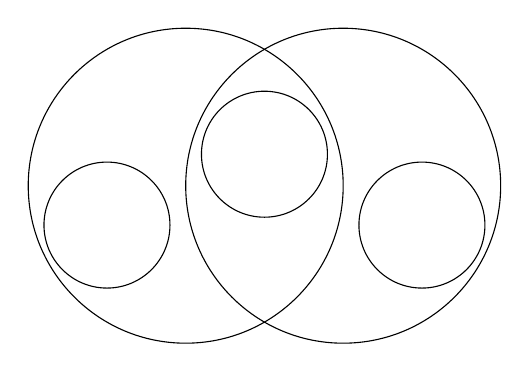
\begin{tikzpicture}
                \def\radius{2cm}

                % some coordinates for the center of the circles
                \coordinate (centerl);
                \coordinate[xshift=-.5*\radius, yshift=-.25*\radius] (centerll);
                \coordinate[xshift=\radius] (centerr);
                \coordinate[xshift=1.5*\radius, yshift=-.25*\radius] (centerrr);
                \coordinate[yshift=.2*\radius, xshift=.5*\radius] (centerm);

                % the circles
                \draw (centerl) circle (\radius);
                \draw (centerr) circle (\radius);
                \draw (centerm) circle (.4*\radius);
                \draw (centerll) circle (.4*\radius);
                \draw (centerrr) circle (.4*\radius);

                %the labels
                \node[xshift=-.5*\radius, yshift=.4*\radius] at (centerl) {$\NP$};
                \node[xshift=.5*\radius, yshift=.4*\radius] at (centerr) {$\coNP$};
                \node at (centerm) {$\pP$};
                \node at (centerll) {$\NPC$};
                \node at (centerrr) {$\coNPC$};
            \end{tikzpicture}
        \end{minipage} vs.
        \begin{minipage}{0.4\textwidth}
            \centering
            \begin{tikzpicture}
                \def\radius{2cm}

                % some coordinates for the center of the circles
                \coordinate (center);

                % \draw  (current bounding box.north west) rectangle (current bounding box.south east);

                % the circles
                \draw (center) circle (\radius);

                %the labels
                \node at (center) {$\pP = \NP = \coNP$};
            \end{tikzpicture}
        \end{minipage}
        \captionof{figure}{Landscape of problems depending if $\pP = \NP$}
    \end{minipage}
\end{openquestion}
\section{Complexity differences between $\IP$ and $\LP$}
Some $\BIP$s are easy, such as bipartite matching, or the assignment problem, even though $\IP \in \NPC$.
In the following section, we want to give intuition, why there are different complexities in $\IP$.
\subsection{Optimization vs. Separation}
\begin{recall}[Ellipsoid Algorithm]
    As discussed in ADM1, the \vocab{ellipsoid method} can be used to determine feasibility of LPs in polynomial time.
    One could also call the ellipsoid method a fancy "$n$-dimensional binary search".
    A rough draft how the algorithm worked:
    \begin{enumerate}
        \item Reduce optimization version to decision version and introduce bound $L = mn \cdot \log(\text{max abs. data})$
        \item Volume-based argument: If the LP is feasible, there is a solution within the centered cube with length $2^L$.
        \item Volume is zero: Perturb the problem to $Ax \leq b + 2^{-L}$, which maintains feasibility, but now has positive volume.
    \end{enumerate}
    For details, refer to the slides from ADM1.
\end{recall}
\begin{definition}
    Given a polyhedron $P$ with an associated cost function. We want to introduce two distinct problem types:
    \begin{itemize}
        \item The \vocab[problem types!optimization]{optimization problem $\mathsf{\OPT}$} denotes the problem of finding an optimal $x^* \in P$.
        \item The \vocab[separation problem]{separation problem $\mathsf{\SEP}$} denotes the problem of deciding if $x \in P$, or else stating a separating hyperplane.
    \end{itemize}
\end{definition}
\begin{remark}
    The key step of the ellipsoid method is to find a hyperplane that separates the current $x$ from the considered polyhedron.
    Especially, if $\SEP \in \pP$, then $\OPT \in \pP$. The converse can also be proven.
\end{remark}
\begin{definition}
    Let $\mathcal{Q}$ be the class of full-dimensional polytopes with $0$ inside.
    We define the \vocab{polar} $Q^*$ for $Q \in \mathcal{Q}$ as
    \begin{align*}
        Q^* \coloneqq \{ y \in \realnum^n \mid \forall x \in Q \colon y^Tx \leq 1  \}.
    \end{align*}
\end{definition}
\begin{theorem}
    Considering this class of polytopes, one can proove \cite[Ch.~4,~Thm.~4.22]{comb-optimization-korte}:
    \begin{enumerate}
        \item $Q^*$ is also a full-dimensional polytope with $0$.
        \item $(Q^*)^* = Q$
        \item $v$ is a vertex of $Q$ iff $v^Ty \leq 1$ is a facet of $Q^*$
    \end{enumerate}
\end{theorem}
\begin{theorem}
    Suppose we can solve $\OPT$ on $\mathcal{Q} \in \pP$ with algorithm $A$.
    Then we can use $A$ as an oracle to solve $\SEP$ on $\mathcal{Q}^*$ in polynomial time.
    \label{thm:sep-opt-lp}
\end{theorem}
\begin{proof}
    Suppose $Q^* \in \mathcal{Q}^*$, and we want to separate $y^0$.
    Use $A$ to solve $\OPT$ on $Q$ with objective function $\max (y^0)^Tx$ to get $x^* \in Q$.
    This yields two cases:
    \begin{itemize}
        \item $(y^0)^Tx^* \leq 1$: Then this holds for all $x \in Q$, and thus $y^0 \in Q^*$ by definition.
        \item $(y^0)^Tx^* > 1$: Consider hyperplane $(x^*)^Ty$. From $x^* \in Q$ it follows that
              for all $y \in Q^*$, that $(x^*)^Ty \leq 1$, but $(x^*)^Ty^0 > 1$. Thus, we found a separating hyperplane.
    \end{itemize}
\end{proof}
\begin{theorem}
    $\SEP \in \pP$ for $\mathcal{Q}$ iff $\OPT \in \pP$ for $\mathcal{Q}$
\end{theorem}
\begin{proof} Using what we proven so far:
    \begin{alignat*}{2}
                                       & \OPT \in \pP \text{ for } \mathcal{Q}   &  & \overset{\ref{thm:sep-opt-lp}}{\IMP}  \SEP \in \pP \text{ for } \mathcal{Q}^*                 \\
        \overset{\text{Ellips.}}{\IMP} & \OPT \in \pP \text{ for } \mathcal{Q}^* &  & \overset{\ref{thm:sep-opt-lp}}{\IMP}  \SEP \in \pP \text{ for } (\mathcal{Q}^*)^*=\mathcal{Q} \\
        \overset{\text{Ellips.}}{\IMP} & \OPT \in \pP \text{ for } \mathcal{Q}
    \end{alignat*}
\end{proof}
\begin{conclusion}
    There is a close relationship between $\OPT$ and $\SEP$:
    \[
        \underset{\OPT}{\framebox[1.1\width]{\text{Complexity}}} \Longleftrightarrow \underset{\SEP}{\framebox[1.1\width]{\text{Integrality}}}
    \]
\end{conclusion}